\documentclass[10pt]{article}
\usepackage{fullpage,enumitem,amsmath,amssymb,graphicx}
\usepackage{tikz}
\usepackage{verbatim}

\begin{document}

\begin{center}
{\Large CS224N Winter 2016 Homework [1]}

\begin{tabular}{rl}
SUNet ID: & [06074217] \\
Name: & [Jiajun Sun] \\
\end{tabular}
\end{center}

By turning in this assignment, I agree by the Stanford honor code and declare
that all of this is my own work.

\section*{Problem 1}
\begin{enumerate}[label=(\alph*)]
\item
The proof is shown as follow:
    \begin{equation*}
    	softmax(x+c)_i=\frac{e^{x_i+c}}{\sum_j e^{x_j+c}}=\frac{e^{x_i}e^c}{\sum_j e^{x_j}e^c}=\frac{e^{x_i}}{\sum_j e^{x_j}}=softmax(x)
    \end{equation*}

\end{enumerate}

\pagebreak[4]
\section*{Problem 2}
\begin{enumerate}[label=(\alph*)]
\item
The gradient of sigmoid function
\begin{equation*}
	\frac{\partial\sigma(x)}{\partial x} = \frac{1}{(1+e^{-x})^2}e^{-x} = \sigma(x)^2(\frac{1}{\sigma(x)}-1) = \sigma(x) - \sigma(x)^2
\end{equation*}
\item
The gradient of cross entropy loss function
\begin{equation*}
	\frac{\partial CE(y,\hat{y})}{\partial\theta} = -\sum_{i}y_{i}\frac{softmax(\theta)'}{\hat{y_{i}}} = -\sum_{i}y_{i}\frac{softmax(\theta)_i'}{softmax(\theta)_i}
\end{equation*}
Consider only the k-th element of $y$ is one:
\begin{equation*}
	\frac{\partial CE(y,\hat{y})}{\partial\theta} = - \frac{softmax(\mathbf{\theta})_k'}{\hat{y}_k}
\end{equation*}
Where,
\begin{equation*}
	\begin{aligned}
	softmax(\mathbf{\theta})_k' & = \frac{\partial softmax(\mathbf{\theta})_k}{\partial\theta_i} = \frac{\partial}{\partial\theta_i}\frac{e^{\theta_{k}}}{\sum_{j}e^{\theta_j}}\\
					 & = \frac{\frac{\partial e^{\theta_k}}{\partial \theta_i}}{\sum_{j}e^{\theta_j}} - e^{\theta_i}\frac{e^{\theta_k}}{(\sum_{j}e^{\theta_j})^2}\\
					 & = \frac{\mathbf{y}e^{\theta_k}}{\sum_{j}e^{\theta_j}} - \frac{e^{\mathbf{\theta}}e^{\theta_k}}{(\sum_{j}e^{\theta_j})^2}\\
					 & = \hat{y}_k(\mathbf{y}-\mathbf{\hat{y}})
	\end{aligned}
\end{equation*}
Therefore,
\begin{equation*}
	\frac{\partial CE(y,\hat{y})}{\partial\theta} = \mathbf{\hat{y}} - \mathbf{y}
\end{equation*}
\item
Use back propogation,
\begin{equation*}
	\frac{\partial J}{\partial \mathbf{x}} = \frac{\partial J}{\partial \mathbf{\hat{y}}}\frac{\partial \mathbf{\hat{y}}}{\partial \mathbf{h}}\frac{{\partial \mathbf{h}}}{\partial \mathbf{x}}
\end{equation*}
first calculate gradient of first two:
\begin{equation*}
	\frac{\partial J}{\partial \mathbf{\hat{y}}}\frac{\partial \mathbf{\hat{y}}}{\partial \mathbf{h}} = \frac{\partial CE(\mathbf{y}, \mathbf{\hat{y}})}{\partial \mathbf{h}} = (\mathbf{\hat{y}} - \mathbf{y})\mathbf{W_2}^T
\end{equation*}
Then calculate the gradient of the hidden layer:
\begin{equation*}
	\frac{\partial \sigma(\mathbf{xW_1}+\mathbf{b_1})}{\partial \mathbf{x}} = \sigma(\mathbf{xW_1}+\mathbf{b_1}))(1-\sigma(\mathbf{xW_1}+\mathbf{b_1})))\mathbf{W_1}^T
\end{equation*}
By combining them together we got:
\begin{equation*}
\begin{aligned}
	\frac{\partial J}{\partial \mathbf{x}} & = [(\mathbf{\hat{y}} - \mathbf{y})\mathbf{W_2}^T][\sigma(\mathbf{xW_1}+\mathbf{b_1}))(1-\sigma(\mathbf{xW_1}+\mathbf{b_1}))]\mathbf{W_1}^T\\
\end{aligned}
\end{equation*}

\item
There are parameters stored in $\mathbf{W_1}$, $\mathbf{W_2}$, $\mathbf{b_1}$, $\mathbf{b_2}$.\\
\\
$\mathbf{W_1}$ has dimension $D_x \times H$\\
$\mathbf{W_2}$ has dimension $D_y \times H$\\
$\mathbf{b_1}$ has dimension $1 \times H$\\
$\mathbf{b_2}$ has dimension $1 \times D_y$\\
\\
Therefore, there are $H(D_y+D_x)+D_y+H$ parameters in this neural network.
\end{enumerate}

\pagebreak[4]
\section*{Problem 3}
\begin{enumerate}[label=(\alph*)]
\item
First denote:
\begin{equation*}
	Z = u^{T}\nu_c
\end{equation*}
Use chain rule to derive the gradient:
\begin{equation*}
	\frac{\partial CE(\mathbf{y}, \mathbf{\hat{y}})}{\partial \nu_c} = \sum_{i}\sum_{j}\frac{\partial CE(\mathbf{y}, \mathbf{\hat{y}})}{\partial \mathbf{\hat{y}}_i}\frac{\partial \mathbf{\hat{y}}_i}{\partial Z_j}\frac{\partial Z_j}{\partial \nu_c}
\end{equation*}
The result should has the same dimension as $\nu_c$ which is $W$. Assume word $o$ is the expected word, therefore, only when index $i = o$ the gradient is not zero:
\begin{equation*}
	\frac{\partial CE(\mathbf{y}, \mathbf{\hat{y}})}{\partial \nu_c} = \sum_{j}\frac{\partial CE(\mathbf{y}, \mathbf{\hat{y}})}{\partial \mathbf{\hat{y}}_o}\frac{\partial \mathbf{\hat{y}}_o}{\partial Z_j}\frac{\partial Z_j}{\partial \nu_c}
\end{equation*}
From problem 2 we know:
\begin{equation*}
	\frac{\partial CE(\mathbf{y}, \mathbf{\hat{y}})}{\partial \mathbf{\hat{y}}_o}\frac{\partial \mathbf{\hat{y}}_o}{\partial Z_j} = (\hat{y}_j - y_j) = (\hat{y}_j - \mathbf{1}[j=o])
\end{equation*}
And it is easy to find:
\begin{equation*}
	\frac{\partial Z_j}{\partial \nu_c} = \mathbf{u}_j
\end{equation*}
Therefore, combine them together:
\begin{equation*}
	\frac{\partial CE(\mathbf{y}, \mathbf{\hat{y}})}{\partial \nu_c} = \sum_j(\hat{y}_j - \mathbf{1}[j=o])\mathbf{u}_j
\end{equation*}

\item
Use chian rule to derive the gradient:
\begin{equation*}
	\frac{\partial CE(\mathbf{y}, \mathbf{\hat{y}})}{\partial u_w} = \sum_{i}\sum_{j}\frac{\partial CE(\mathbf{y}, \mathbf{\hat{y}})}{\partial \mathbf{\hat{y}}_i}\frac{\partial \mathbf{\hat{y}}_i}{\partial Z_j}\frac{\partial Z_j}{\partial u_w}
\end{equation*}
It is easy to find that index $i=o$ and $j=w$ the gradient is not zero:
\begin{equation*}
	\frac{\partial CE(\mathbf{y}, \mathbf{\hat{y}})}{\partial u_w} = \frac{\partial CE(\mathbf{y}, \mathbf{\hat{y}})}{\partial \mathbf{\hat{y}}_i}\frac{\partial \mathbf{\hat{y}}_i}{\partial Z_w}\frac{\partial Z_w}{\partial u_w}
\end{equation*}
\begin{equation*}
	\frac{\partial CE(\mathbf{y}, \mathbf{\hat{y}})}{\partial \mathbf{\hat{y}}_o}\frac{\partial \mathbf{\hat{y}}_o}{\partial Z_w} = (\mathbf{\hat{y}_w} - \mathbf{y_w}) = (\mathbf{\hat{y}_w} - \mathbf{1}[w=o])
\end{equation*}

\begin{equation*}
	\frac{\partial Z_w}{\partial u_w} = \mathbf{\nu_c}
\end{equation*}
Therefore, combine them together:
\begin{equation*}
	\frac{\partial CE(\mathbf{y}, \mathbf{\hat{y}})}{\partial u_w} = (\mathbf{\hat{y}_w} - \mathbf{1}[w=o])\mathbf{\nu_c}
\end{equation*}

\item
Gradient for $\nu_c$:
\begin{equation*}
\begin{aligned}
	\frac{\partial J}{\partial \nu_c} & = -\frac{\frac{\partial \sigma(u_o^T\nu_c)}{\partial \nu_c}}{\sigma(u_o^T\nu_c)} - \sum_k \frac{\frac{\partial \sigma(-u_k^T\nu_c)}{\partial \nu_c}}{\sigma(-u_k^T\nu_c)}\\
	& = -\frac{\sigma(u_o^T\nu_c)(1-\sigma(u_o^T\nu_c))u_o}{\sigma(u_o^T\nu_c)} - \sum_k \frac{\sigma(-u_k^T\nu_c)(1-\sigma(-u_k^T\nu_c))(-u_k)}{\sigma(-u_k^T\nu_c)}\\
	& = (\sigma(u_o^T\nu_c)-1)u_o + \sum_{k, k\neq o}(1-\sigma(-u_k^T\nu_c))u_k
\end{aligned}
\end{equation*}

Gradient for $u_w$:

\begin{equation*}
\begin{aligned}
	\frac{\partial J}{\partial u_w} & = -\frac{\frac{\partial \sigma(u_o^T\nu_c)}{\partial u_w}}{\sigma(u_o^T\nu_c)} - \sum_k \frac{\frac{\partial \sigma(-u_k^T\nu_c)}{\partial u_w}}{\sigma(-u_k^T\nu_c)}\\
	& = -\mathbf{1}[o=w]\frac{\sigma(u_o^T\nu_c)(1-\sigma(u_o^T\nu_c))u_o}{\sigma(u_o^T\nu_c)} - \mathbf{1}[o\neq w]\frac{\sigma(-u_w^T\nu_c)(1-\sigma(-u_w^T\nu_c))(-\nu_c)}{\sigma(-u_w^T\nu_c)}\\
	& = \mathbf{1}[o=w](\sigma(u_o^T\nu_c)-1)\nu_c + \mathbf{1}[o\neq w](1-\sigma(-u_w^T\nu_c))\nu_c
\end{aligned}
\end{equation*}
when $o=w$
\begin{equation}
\frac{\partial J}{\partial u_0} = (\sigma(u_o^T\nu_c)-1)\nu_c
\end{equation}

when $o\neq w$
\begin{equation}
\frac{\partial J}{\partial u_w} = (1-\sigma(-u_w^T\nu_c))\nu_c
\end{equation}

\item
In skip-gram, we use the center word to predict context words, then we take gradient W.R.T $\nu_c$:
\begin{equation*}
\begin{aligned}
	\frac{\partial J_{skip-gram}(word_{c-m...c+m})}{\partial \nu_{c}} & = \sum_{-m\le j\le m, j\neq0} \frac{\partial F(w_{c+j}, \nu_c)}{\partial \nu_{c}}\\
\end{aligned}
\end{equation*}
\begin{equation*}
\begin{aligned}
	\frac{\partial J_{skip-gram}(word_{c-m...c+m})}{\partial \nu_{k}} & = 0, k\neq c\\
\end{aligned}
\end{equation*}

In CBOW, the predicted vector contain all input vectors of that corpus, therefore take gradient W.R.T to $\nu_{c+j}$:
\begin{equation*}
\begin{aligned}
	\frac{\partial J_{CBOW}(word_{c-m...c+m})}{\partial \nu_{c+j}} & = \frac{\partial F(w_{c}, \hat{\nu})}{\partial \hat{\nu}}\\
\end{aligned}
\end{equation*}
\begin{equation*}
\begin{aligned}
	\frac{\partial J_{CBOW}(word_{c-m...c+m})}{\partial \nu_{c+k}} & = 0, k\notin[-m, m]\\
\end{aligned}
\end{equation*}

\begin{figure}[h]
\center
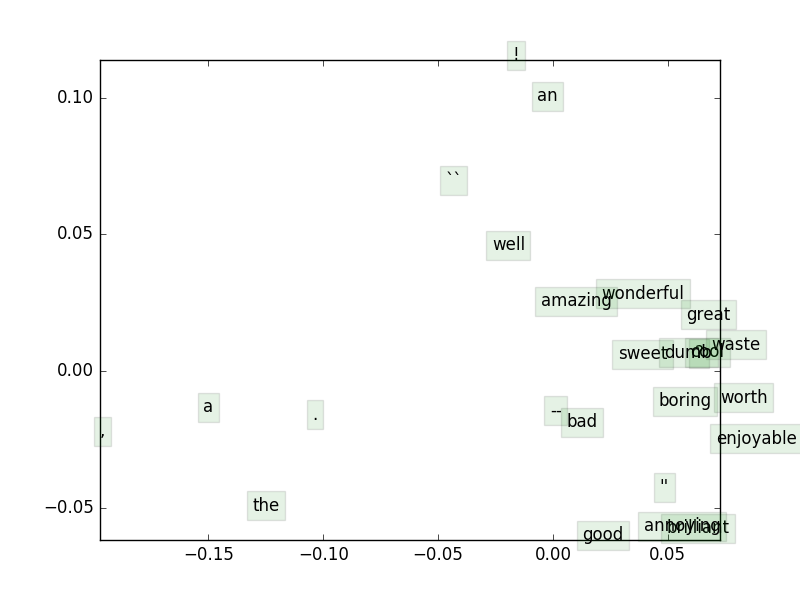
\includegraphics[scale=0.5]{q3_word_vectors.png}
\end{figure}
\item
In the above plot we can see: most adjective word convey sentiment meanings are clustered together.
This plot shows the different roles a word play in a sentence.
If visulise more dimensions, we can expect the seperation of different adjective words.


\end{enumerate}

\pagebreak[4]
\section*{Problem 4}
\begin{enumerate}[label=(\alph*)]
\item
\item
By adding regularization is to prevent overfitting.
Regularization by adding penaties to the norm of estimates can limit the variance of the model with a compromise on the training error.

\item
\verbatiminput{chooseBestModel.txt}

\item
For pretrained vector, when regularization value is $12.1$, the train, dev and test are $38.659$, $37.148$ and $37.557$ respectively.\\
For our own vector, when regularization value is $2.61E-06$, the train, dev and test are $31.016$, $32.698$ and $30.271$ respectively.\\
\\
The best results are listed in the table below:\\
\\
\begin{tabular}{ l | c | r }
\centering
        & Pretrained & your-vectors \\ \hline
  train & 39.958 & 31.180 \\ \hline
  test  & 37.148 & 32.698 \\ \hline
  dev   & 37.557 & 30.271 \\ \hline
\end{tabular}
\\
There are three reasons that Pretrained vectors has higher accuracy:\\
\\
(1) GloVe combine $u$ and $v$,
therefore the vector it generates might be more representative than word2vec methods.\\
(2) Pretrained and the vectors we trained use different datasets.
Wikipedia may have larger vacabulary sets than SST datasets.
As a result, word vectors trained from Wikipedia will contain more meanings and more comprehensive.\\
(3) When training our own word vectors we use a one layer model,
this model could be simpler than how GloVe vector was trained.
By implementing a deeper layer model might increase the accuracy of our word vectors.


\item
Both train and dev accuracy decrease with the increase of regularization parameters.
With higher regularization value, the regularization parameter $C$ for logistic regreesion become smaller.
As described in sklearn, smaller $C$ means stronger regularization strength. This will lead model underfitting.

\begin{figure}[h]
\center
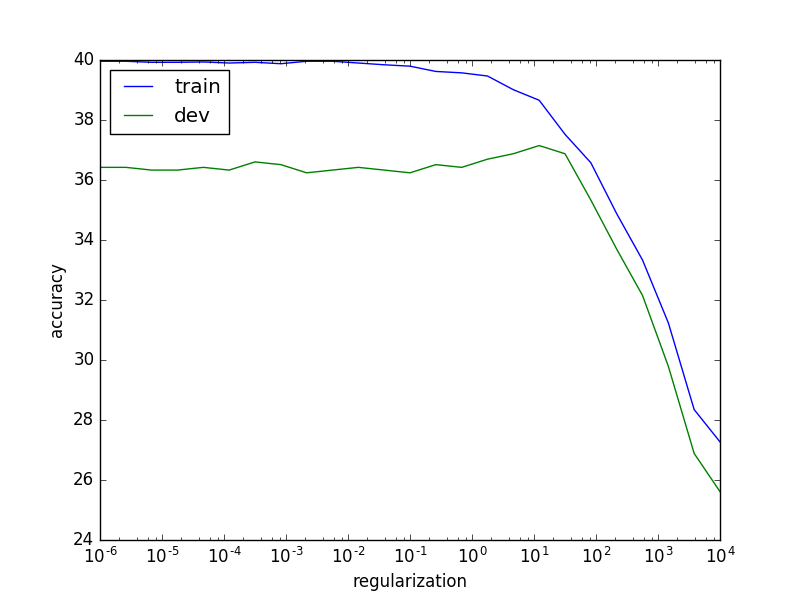
\includegraphics[scale=0.5]{q4_reg_v_acc.png}
\end{figure}

\item
Prediction on positive meaning and negative meaning are relative balanced but slightly towards the positive side.
Our model does not have enough variance to predict the true label.
Most of the prediction falls on eight moderate positive or moderate negative.
\begin{figure}[h]
\center
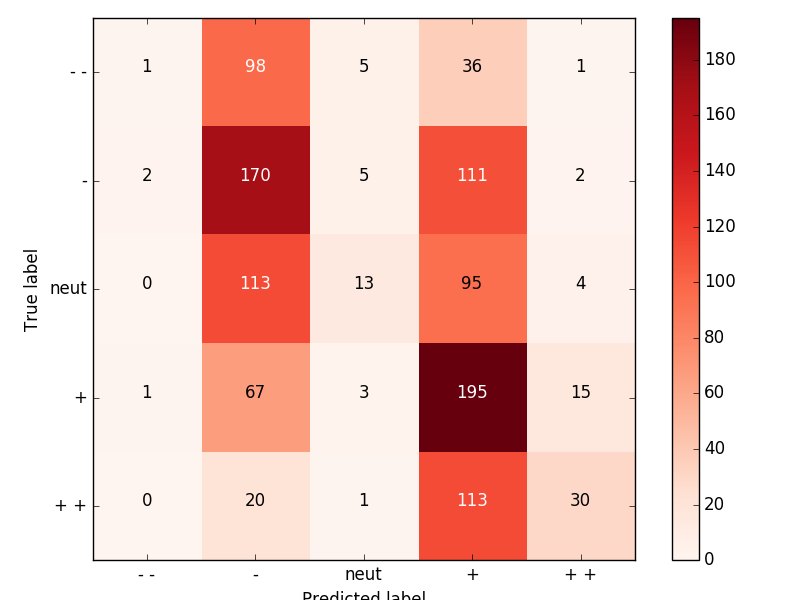
\includegraphics[scale=0.5]{q4_dev_conf.png}
\end{figure}


\item
\textbf{Example 1: 3	1	we know the plot 's a little crazy , but it held my interest from start to finish.}\\
The word "crazy" has convey too much negative meaning,
however the sentiment analysis does not consider the "but" which flip the meaning of the sentence.\\
\\\textbf{Example 2: 3	1	not far beneath the surface , this reconfigured tale asks disturbing questions about those things we expect from military epics.}\\
This sentence`s meaning is not obvious. By adding up all vector can not figure out the meaning\\
\\\textbf{Example 3: 4 1	manages to transcend the sex , drugs and show-tunes plot into something far richer.}\\
Here transcend should have more weights than other words.
\end{enumerate}

\end{document}

